\section{Notation and problems}
\label{sec:prelim}
Let $G = (V, E)$ be a contact graph where $V$ is the set of people (or nodes) and $e = (u, v) \in E$ if nodes $u, v \in V$ come into direct contact, which can allow a disease to spread. Let $n = |V|$ be the number of nodes in graph $G$. 
We assume a simple SIR model of disease spread \cite{marathe:cacm13}, in which each node is in one of the following states:
susceptible (S), infectious (I) or recovered (R).
The epidemic starts at one or more externally infected nodes, and spreads from an infected node $u$ to each susceptible
neighbor $v$ with probability $p$. An infected node becomes recovered in the next time step.
We assume $s_v$ is the probability that $v$ is initially infected; $\mathbf{s}$ denotes the initial infection vector.
As is typical in public health analyses, we will assume a small number of random initial infections.
We note that there are lots of variations of the SIR model, such as:
varying transmission probability $p(u, v)$ on each edge $(u, v)$,
with an exposed state, varying infectious duration, etc.;
most of our results extend to the general models.

\begin{figure}
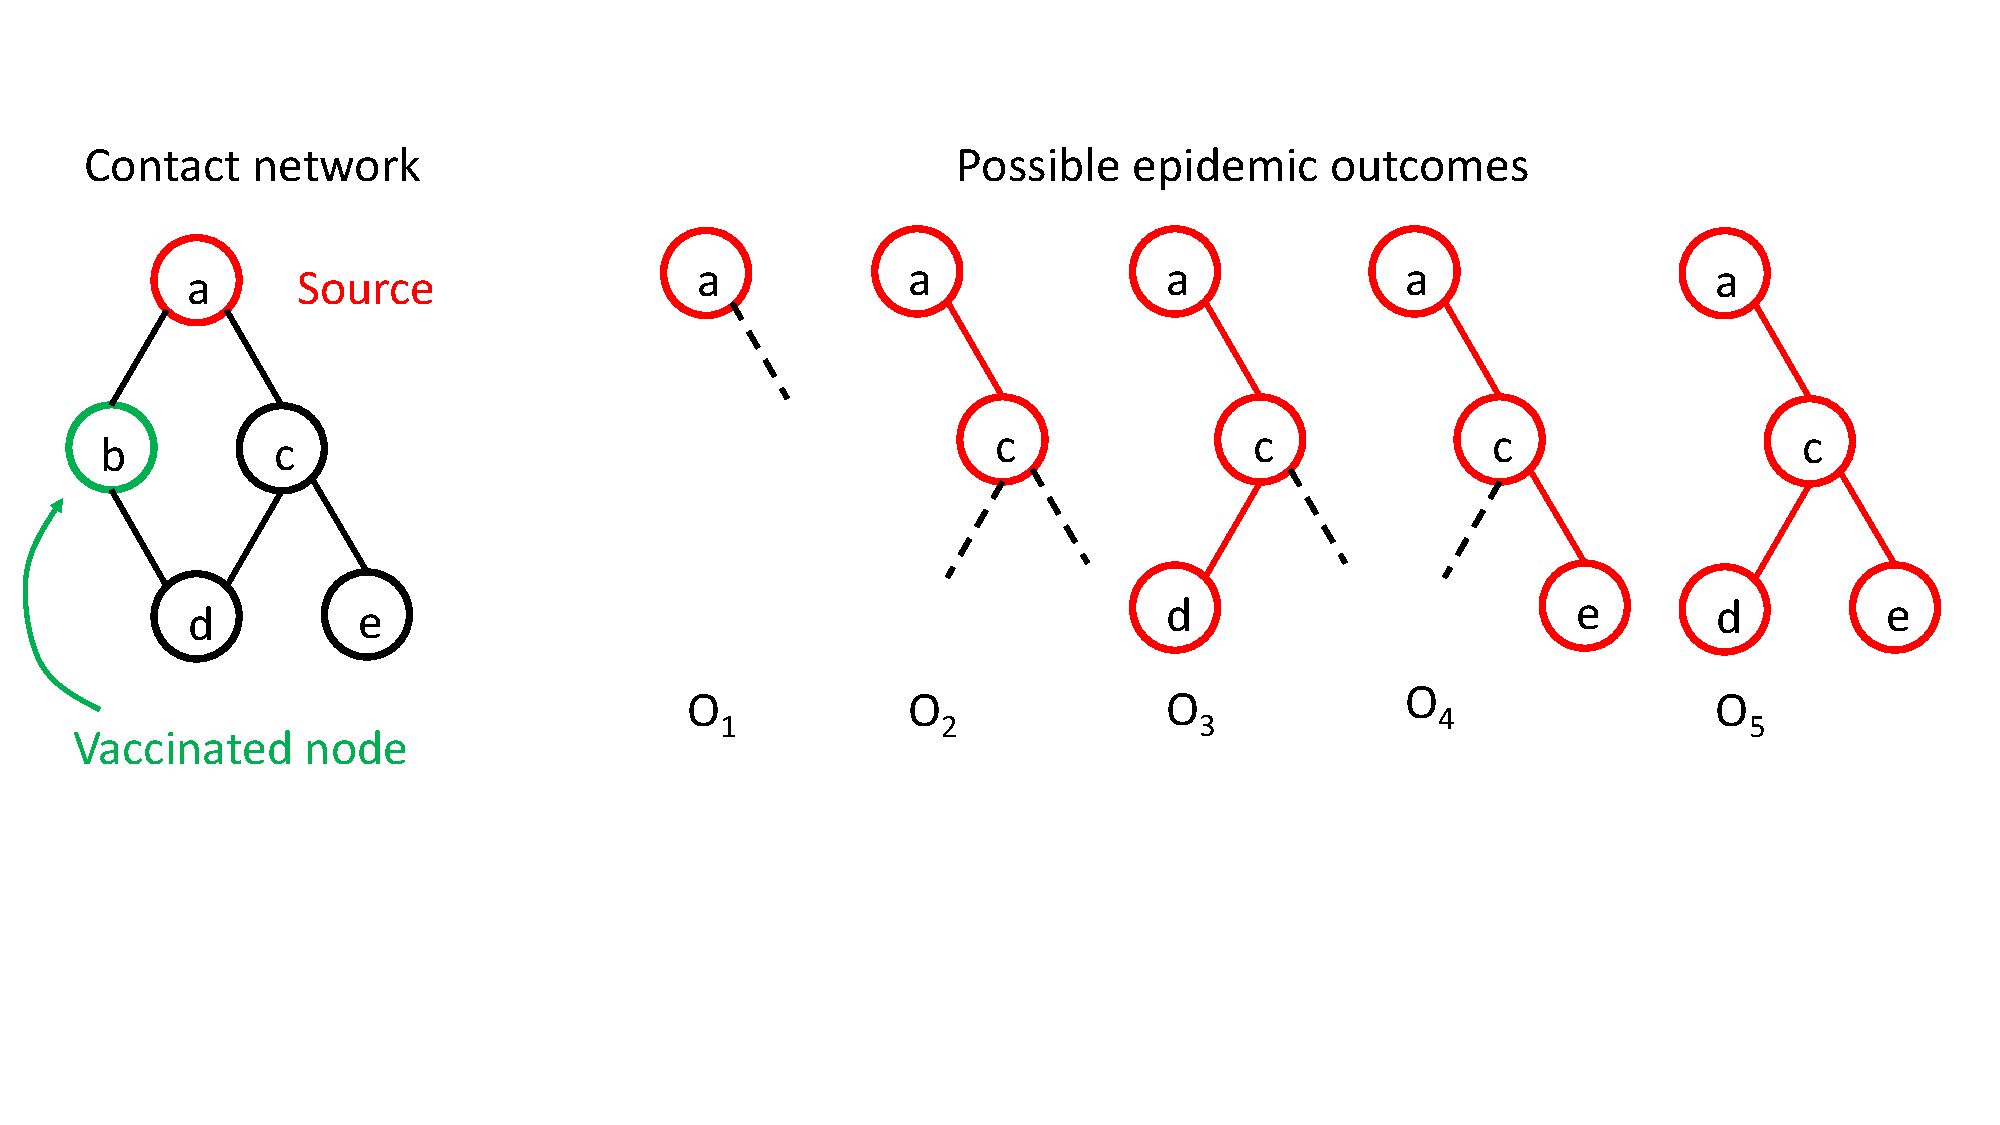
\includegraphics[scale=0.25]{figures/example.pdf}
\caption{Example illustrating the SIR model: the contact network $G=(V, E)$ is shown in the left,
with $V=\{a, b, c, d, e\}$ (shown in circles), and edges as solid lines.
Node $a$ is initially infected, and node $b$ is vaccinated. The five subgraphs $O_1, O_2, O_3, O_4, O_5$
(on the right) are possible stochastic outcomes in the SIR model.}
\label{fig:example}
\end{figure}

We use $x_{vt}$ as an indicator variable, which is $1$ if node $v$ gets vaccinated at time $t$.
Let $\X_t=\{v: x_{vt}=1, v\in V\}$ denote the set of nodes vaccinated at time $t$, and 
$\X=\{\X_t: t\in\mathcal{T}\}$ denote the combined set of all temporal vaccination
decisions; here $\mathcal{T}=\{t_0, t_1,\ldots\}$ denotes a set of times at which decisions are to be made.
We assume the vaccine is immediately effective; our methods can be extended to handle limited efficacy vaccines.
We assume a budget vector $\B=(B_t: t\in\mathcal{T})$, which specifies the number of vaccines available
at each time $t\in\mathcal{T}$.
Let $\expinf(G, \src, \mathcal{T}, \X)$ denote the expected number of infections that occur if the epidemic
starts with the vector $\src$, and nodes are vaccinated at each time $t\in\mathcal{T}$, as per the vector $\X_t$.
When the inputs are clear from the context, we just refer to this as $\expinf(\X)$.

\noindent
\textbf{Example.} Figure \ref{fig:example} shows the SIR model and the definitions of the above quantities
on a graph $G$ with five nodes. Initially, node $a$ is infected, and $b$ is vaccinated. 
In the SIR model, the disease spreads from an infected node to each susceptible neighbor with probability $p$,
and does not spread with probability $1-p$. Therefore, we have five possible stochastic outcomes $O_1,\ldots,O_5$,
which occur with probabilities $1-p$, $p(1-p)^2$, $p^2(1-p)$, $p^2(1-p)$, and $p^3$, respectively.
Suppose we have $\mathcal{T}=\{0\}$. Then, $x_{b0}=1$, and $\X=\X_0=\{b\}$.
We have 
\[
\expinf(\X)= (1-p) +2p(1-p)^2+2\cdot 3 p^2(1-p) + 4p^3
\]

\noindent
\textbf{The temporal vaccination problem (\prob).}\\
\underline{Given}: contact network $G=(V, E)$, initial infection vector $\mathbf{s}$, set of times $\mathcal{T}$,
budget vector $(B_t: t\in\mathcal{T})$\\
\underline{Compute}: a set $\X$ of intervention sets at each time, 
such that $\expinf(G, \src, \mathcal{T}, \X)$ is minimized, and $\sum_v x_{vt} \leq B_t$ for all $t\in\mathcal{T}$.


The formulation of \prob{} does not involve any information of the epidemic spread at an intermediate
time, and all decisions are made ahead of time. Therefore, this problem is non-adaptive, and no information
about the state of the outbreak is used. We now study a different formulation, which allows information about
the outbreak, and a delay $\tau$ in availability of this information. Let $I_t$ be the set of nodes that
get infected at time $t$.
We consider an intervention at time $T$, with all information about the outbreak till time $T-\tau$ being available,
namely the set $\info=\{I_t: t\leq T-\tau\}$; note that the set $I_0$ is precisely the set of sources of infection.
For a set $\X_T$ of vaccinated nodes, and set $\info$, let $\expinf(G, T, \tau, \info, \X_T)$ denote the expected size of
resulting outbreak. 

\noindent
\textbf{Intervention design with delay problem (\probdelay)}\\
\underline{Given}: contact network $G=(V, E)$, information about outbreak $\info$, time $T$, delay $\tau$,
budget $B_T$\\
\underline{Compute}: a feasible set $\X_T$ of nodes to vaccinate at time $T$,
such that $\expinf(G, T, \tau, \info, \X_T)$ is minimized, and $|\X_T|\leq B_T$.
